\documentclass{beamer}
 
 \usepackage{graphicx}
 
% \usepackage{beamerthemesplit} % // Activate for custom appearance

\usetheme{Frankfurt}

\usefonttheme[hoptionsi]{serif}

\title{Feature Model Bad Smells}

\subtitle{Initial catalog and mining tools}

\author{Rodrigo Bonif\'{a}cio \and Leopoldo Teixeira \and Paulo Borba \\ \and Rohit Gheyi \and Tiago Massoni}

\date{\today}

\begin{document}

\frame{\titlepage}

\section{Context}

\begin{frame}
  \frametitle{Feature modeling}
  
\begin{center}
  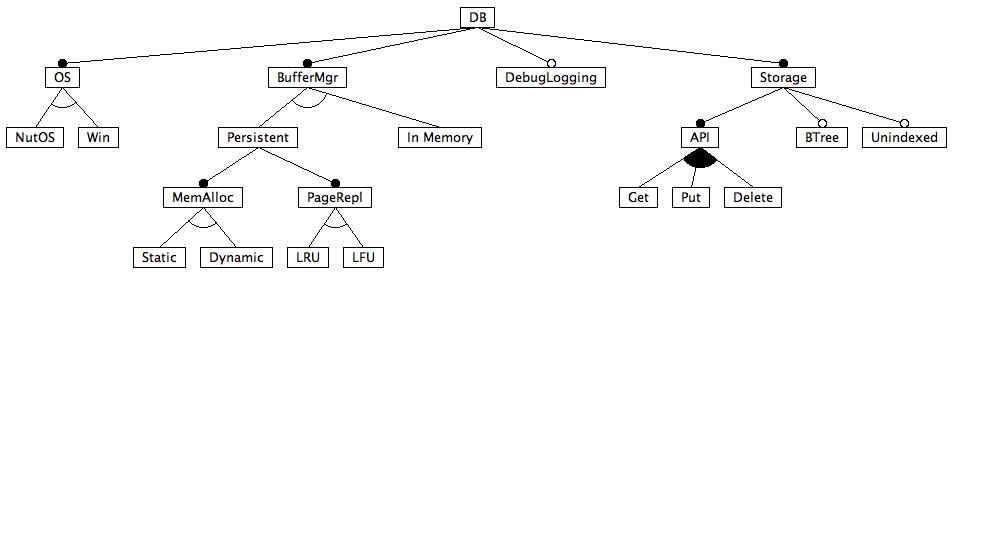
\includegraphics[scale=0.38]{images/berkley-fm.eps} % requires the graphicx package
\end{center}

\begin{small} 

Additional constraints

\begin{enumerate}
 \item  $(Storage \Rightarrow BTree \lor Unindexed) \land \lnot(BTree \land Unindexed)) $
 \item $DebugLogging \Rightarrow Persistent$
 \item \ldots
\end{enumerate}

\end{small}

\end{frame}

\begin{frame}

\frametitle{Although a very simple semantic, ...}

According to Gheyi et al.

\begin{quote}
The semantics of a FM is the set of its possible (valid) configurations. 
A configuration contains a set of feature names; if valid, it satisfies all
constraints (relations and formulas) of the model.
\end{quote}

\end{frame}

\begin{frame}

\frametitle{... being easily reduced to propositional formulas...}

\begin{small}
\begin{itemize}
 \item $DB$ 
 \item $(DB \Leftrightarrow OS) \land (DB \Leftrightarrow BufferMgr) \land (DB \Leftrightarrow Storage)$
 \item $(OS \Rightarrow (NutOS \oplus Win)) \land \ldots \land (DebugLogging \Rightarrow DB)$ 
 \item $(API \Rightarrow (Get \lor Put \lor Delete))$
 \item \ldots
 \item $(Storage \Rightarrow BTree \lor Unindexed) \land \lnot(BTree \land Unindexed)) $
\end{itemize}
\end{small}

\end{frame}

\begin{frame}

\frametitle{... feature modeling still lacks}

\begin{enumerate}
\item a precise notion of type correctness
\item some guidance for avoiding bad design decisions
\item tools for detecting and fixing these kinds of pitfalls 
\end{enumerate}

\end{frame}

\begin{frame}

\frametitle{Existing works}

Benavides and others (VAMOS'07)
\begin{itemize}
\item A feature model {\bf is valid} when do exists at least one product satisfying all 
of its relationships and constraints.  
\end{itemize}

\end{frame}

\begin{frame}

\frametitle{Is this feature model correct?}

\begin{center}
  \includegraphics[scale=0.4]{images/fm-linux.eps} 
\end{center}
\begin{small}
\begin{enumerate}
\item $USE\_GENERIC\_SMP\_HELPERS \Rightarrow SMP$
\item $USE\_GENERIC\_SMP\_HELPERS \Rightarrow SMP$
\item \ldots
\item $M386 \Rightarrow (X86\_32 \land (\lnot UML)) \bullet UML \notin features (Linux) $
\end{enumerate}
\end{small}
\end{frame}

\begin{frame}

\frametitle{Existing works}

Thomas von der Ma$\beta$en and Horst Lichter (SPFE'04)

\begin{itemize}
\item Recommend the development of \emph{consistency checkerers} for feature modeling.   
\item Propose a tool that checks a {\bf small set of properties} between features and requirements.
\item The paper focuses on irrelevant decisions of the tool and does not detail which properties (and how they) are checked.
\end{itemize}

\end{frame}

\begin{frame}

\frametitle{Existing works}

Krzysztof Czarnecki and Chang Hwan Peter Kim \\ (OOPSLA'05 Workshop on Software Factories )

\begin{itemize}
\item Propose the use of BDDs for checking:
\begin{itemize}
\item constraints, propagation, satisfiability
\item dead features
\item the number of valid configurations
\end{itemize}
\end{itemize}

\end{frame}

\begin{frame}

\frametitle{Existing works}

P. Trinidad and others \\ (Journal of Systems and Software, 2007)

\begin{itemize}
\item Claim for \emph{error-free} feature models
\item Check a few properties using \emph{Theory of Diagnosis} 
\begin{itemize}
 \item dead features
 \item full-mandatory features
 \item void feature models 
\end{itemize}
\end{itemize}

\end{frame}


\begin{frame}
\frametitle{In summary}

\begin{itemize}
\item Existing works focus on satisfiability issues
\item Other properties are miss considered

\begin{itemize}
 \item correctness
  \item legibility
  \item redundancy
 \end{itemize} 
\item There is no tool for detecting and proposing feature model refactorings

\end{itemize}

\end{frame}

\section[Outline]{}

\frame{\tableofcontents}

\section{Bad smells}

\begin{frame}

\frametitle{Redundant constraint}

\begin{center}
  \includegraphics[scale=0.55]{images/fm-linux-arch.eps}

$64BIT \Rightarrow ARCH$

\end{center}

{\bf Proposed refactoring:} remove constraint
\end{frame}

\begin{frame}

\frametitle{Expecting multiple alternatives}

\begin{center}
  \includegraphics[scale=0.50]{images/berkley-db-missing-alternative.eps}
\end{center}

{\bf Proposed refactoring:} replace alternative to mandatory


\end{frame}

\section{Evaluation}

\section{Next steps}

\end{document}
